% =====================================================================================
\section{Method}
\label{sec:method}

\paragraph{Overview.} A frozen pretrained language model learns $T$ tasks one after another. Each
task gets its own small low-rank adapter, which is never changed after its task has been
learned. At test time the model is not told the task of an input. A \emph{switch} sends
every input to one task, and the model answers as it was when that task was
learned. An answer can then change only if the switch changes its route (Lemma~\ref{lem:route}),
so everything that can be said about forgetting is a statement about the rule that sets the route.
We call the whole system FK-LoRA, after the rule \emph{finders keepers}.
Three rules are given. The first, which we recommend, reads no instruction: \recog{}, a
\emph{recogniser} over all tasks on frozen states of the model itself, which blocks no task, with
an audit of the changed answers from held-out inputs and, in its variant \handicap{}, a bound in advance on what a later task
can take (Section~\ref{sec:audit}). The second, \cert{}, applies when every input carries the instruction of
its task: each task owns a \emph{protected zone} around the frozen word-vectors of its instruction,
an input inside a zone belongs to the oldest task that claims it, its answer can never change
again, and the system returns a certificate with the answer
(Sections~\ref{sec:features}--\ref{sec:guarantee}). The third builds such zones from the inputs of a
task instead of its instruction; its bound does not grow with the number of later tasks, but in our
tests it blocked later tasks (Section~\ref{sec:bound}). Statements that are not needed to follow the
argument are proved in Appendix~\ref{app:methoddetails}. Figure~\ref{fig:overview} sets this beside one shared adapter and beside the two published methods we ran, and Figure~\ref{fig:switch} shows the three rules.

\begin{figure}[t]
  \centering
  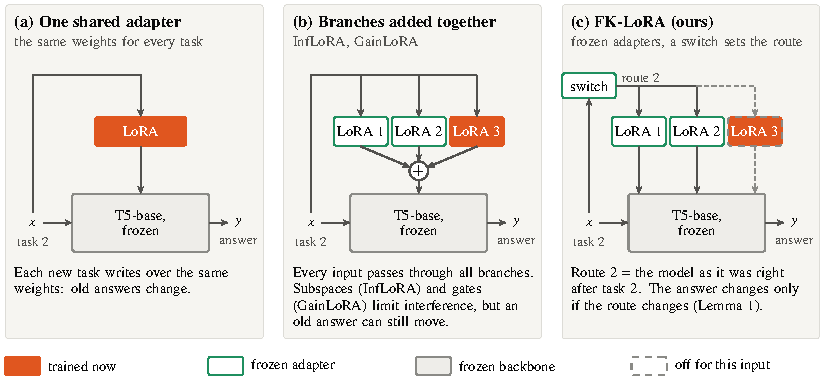
\includegraphics[width=\linewidth]{figures/overview}
  \caption{Three ways to add a task, shown while task~3 is being learned and an input of task~2 is
  answered. (a)~One shared adapter is trained again for each task, so old answers change.
  (b)~InfLoRA and GainLoRA add one branch per task, and every input passes through all branches
  (weighted by gates in GainLoRA); a chosen subspace or the gates limit what a new branch does to
  old inputs, but an old answer can still change. (c)~FK-LoRA never changes an adapter after its
  task has been learned, and a switch sets the route of each input: route~2 is the model as it was
  right after task~2, so the answer changes only if the route changes (Lemma~\ref{lem:route}).}
  \label{fig:overview}
\end{figure}


\subsection{Setting: adapters, routes and answers}
\label{sec:setting}

Let $\mathcal{V}$ be the vocabulary and $E \in \R^{|\mathcal{V}| \times d}$ the input embedding
table of the base model; $E$ and all other base weights $\theta_0$ are frozen. An input is a
sequence of tokens $x = (x_1, \dots, x_L)$. Task $k$ adds a LoRA adapter \citep{hu2022lora} to every adapted weight matrix $W_0$ of the base
model, $\Delta W_k = \tfrac{\alpha}{r} B_k A_k$ with rank $r$. After $T$ tasks an adapted layer
computes
\begin{equation}
  h \;=\; \Bigl( W_0 + \sum_{k=1}^{T} g_k(x)\, \Delta W_k \Bigr) z ,
  \qquad g_k(x) \in \{0, 1\},
  \label{eq:layer}
\end{equation}
where $z$ is the input of the layer and $g_k(x)$ switches adapter $k$ on or off for the whole input
$x$, in every adapted layer. The methods of this paper differ only in the switches. All of
them use a \emph{route} $\rho_T(x) \in \{1, \dots, T\}$ and set
\begin{equation}
  g_k(x) \;=\; \mathbf{1}\bigl[\, k \le \rho_T(x) \,\bigr] ,
  \label{eq:gates}
\end{equation}
so an input with route $j$ is processed with the adapters of tasks $1, \dots, j$,
the model as it was right after task $j$ had been learned. The answer after $T$ tasks is
\begin{equation}
  y_T(x) \;=\; F\bigl(x;\; \theta_0,\; \{A_k, B_k\}_{k \le \rho_T(x)}\bigr),
  \label{eq:answer}
\end{equation}
where $F$ runs the model with a deterministic decoding rule (greedy in all our experiments).

\begin{lemma}[An answer changes only with its route]
\label{lem:route}
Assume that the adapters of a task are never changed after the task has been learned, that the
base model, its tokenizer, the input template and truncation are fixed, and that decoding is
deterministic. Then for every rule that sets the route, every input $x$ and all times $T' > T$:
if $\rho_{T'}(x) = \rho_T(x)$, then $y_{T'}(x) = y_T(x)$.
\end{lemma}

\begin{proof}
Let $j = \rho_T(x) = \rho_{T'}(x)$, so $j \le T$. By Eq.~\eqref{eq:answer} both answers are
$F(x; \theta_0, \{A_k, B_k\}_{k \le j})$. The adapters of the tasks $1, \dots, j$ exist at time $T$
and are the same at time $T'$, and $F$ is deterministic.
\end{proof}

The lemma uses nothing about the model except that it is a deterministic function of its input and
of the adapters that are switched on. It turns retention into a property of the route.

\begin{figure}[t]
  \centering
  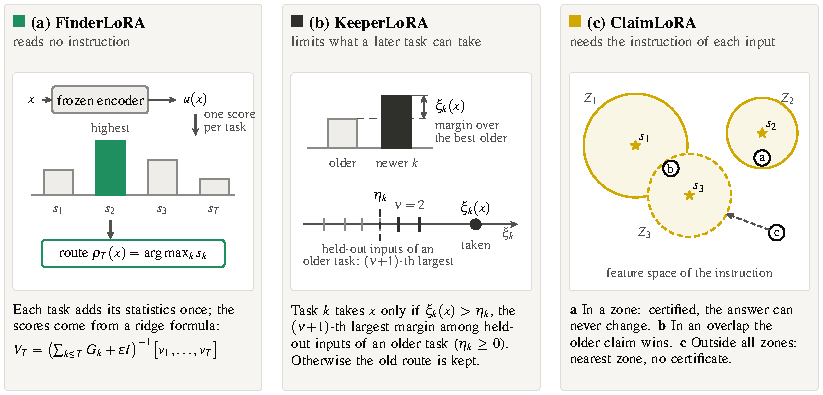
\includegraphics[width=\linewidth]{figures/switch}
  \caption{The three rules that set the route. (a)~\recog{} reads no instruction: it scores every
  task on a frozen feature $u(x)$ of the input with one ridge formula and takes the highest score.
  (b)~\handicap{} adds a handicap for a new task: task $k$ takes an input only if its margin
  $\xi_k(x)$ over the best older task is above $\eta_k$, the $(\nu+1)$-th largest margin among the
  held-out inputs of an older task ($\nu = 2$ in our runs). (c)~\cert{} needs the instruction of
  each input: a task owns a protected zone around the signature of its instruction; an input in a
  zone is certified and belongs to the oldest zone that contains it, and an input outside every
  zone goes to the nearest zone without a certificate.}
  \label{fig:switch}
\end{figure}


% =====================================================================================
\subsection{Without instructions: a recogniser, an audit, and a handicap}
\label{sec:audit}

One classifier over all tasks decides the route from a frozen feature of the whole input, so no
task can be blocked and nothing has to be known about how a task is worded. Its guarantees are
an \emph{audit}, an estimate and a confidence bound from held-out inputs of the share of a task's
answers that have changed, and a \emph{handicap}, a limit known in advance on what a later task
can take from an older one. The audit is ordinary held-out estimation and the handicap a conformal
rank argument with a union bound; what is new is that, by Lemma~\ref{lem:route}, both become
statements about answers.

\paragraph{The price of having no instruction.} For any system whose answer depends on the input alone, two tasks whose inputs overlap
cannot both be answered well: what the older task loses plus what the newer one loses is at least
a conflict $\Omega_{jk}$, the overlap of the two input distributions weighted by how much the best
answers differ (Proposition~\ref{prop:noinstructionprice}). If no input belongs to both tasks,
nothing is forced; this is the exact sense in which an instruction gives the task away. A switch
can only choose how the loss is split: the zones put it on the newer task, \recog{} and
\handicap{} a measured or limited part of it on the older one.

\paragraph{A joint recogniser.} Let $u(x) \in \mathbb{R}^d$ be a frozen feature of the whole
input (the mean of the last-layer states of the frozen encoder of the base
model, without adapter, standardised with the mean and standard deviation of a fixed pool of
instances of other tasks, Section~\ref{sec:protocol}), and
$\bar u(x) = (u(x), 1)$. When task $k$ arrives, its
training inputs are split at random into fit inputs $D_k^{\mathrm{f}}$ and $m$ held-out inputs
$c_1, \dots, c_m$. With $G_k = |D_k^{\mathrm{f}}|^{-1} \sum_{x \in D_k^{\mathrm{f}}} \bar u(x)\, \bar u(x)^{\!\top}$ and $v_k = |D_k^{\mathrm{f}}|^{-1} \sum_{x \in D_k^{\mathrm{f}}} \bar u(x)$ (so every task has the same weight),
the recogniser after $T$ tasks is
\begin{equation}
  V_T \;=\; \Bigl(\, \sum_{k \le T} G_k + \varepsilon\, I \Bigr)^{-1} \bigl[\, v_1, \dots, v_T \,\bigr]
  \label{eq:recogniser}
\end{equation}
with a fixed $\varepsilon > 0$, and the route of an input is the task with the largest score, the older task in a tie,
\begin{equation}
  \rho_T(x) \;=\; \arg\max_{k \le T}\ \bigl(\bar u(x)^{\!\top} V_T\bigr)_k .
  \label{eq:jointroute}
\end{equation}
$V_T$ is the ridge regression of the task labels on the features of all tasks seen so far. The
sums are only added, so it is the same for every order of arrival, no input is kept, and every task
has a column of its own: no task is blocked. The adapter of a task may be trained on all of its
inputs, the held-out ones included; the recogniser never sees those. Such a recogniser is known
from class-incremental learning on frozen features \citep{mcdonnell2023ranpac,zhuang2022acil}; what
we add is what is said about its routes.

\begin{proposition}[An audit of forgetting from held-out inputs]
\label{prop:audit}
Fix a task $j$ and two times $T' > T \ge j$. Let the fit inputs of all tasks and the choice of the
later tasks be independent of the held-out inputs $c_1, \dots, c_m$ of task $j$ and of a further
input $X$ of task $j$, let the route at every time be fitted without them (as in
Eqs.~\eqref{eq:recogniser}--\eqref{eq:jointroute}), and let $c_1, \dots, c_m, X$ be exchangeable
given everything else. Let $H$ be the number of held-out inputs with
$\rho_{T'}(c_i) \ne \rho_T(c_i)$. Then
\[
  \Pr\bigl[\, y_{T'}(X) \ne y_T(X) \,\bigr] \;\le\; \Pr\bigl[\, \rho_{T'}(X) \ne \rho_T(X) \,\bigr]
  \;=\; \mathbb{E}\Bigl[\frac{H}{m}\Bigr] .
\]
If the inputs are independent draws, then with probability at least $1 - \delta$ over the held-out
inputs, the share of the inputs of task $j$ whose route differs between $T$ and $T'$ is at most
the one-sided Clopper--Pearson upper bound for $H$ successes in $m$ trials at confidence
$1 - \delta$. Both statements also hold when ``differs between $T$ and $T'$'' is replaced by ``is
not the same at all times from $T$ to $T'$'', with $H$ counted in the same way.
\end{proposition}

\begin{proof}
The first inequality holds input by input, by Lemma~\ref{lem:route}. Let
$I(x) = \mathbf{1}[\rho_{T'}(x) \ne \rho_T(x)]$. Given everything but $c_1, \dots, c_m, X$ the two
routes are fixed functions, so $I(c_1), \dots, I(c_m), I(X)$ are exchangeable
and $\Pr[I(X) = 1] = \mathbb{E}[I(c_i)] = \mathbb{E}[H]/m$. For independent draws, $H$ is, given
the routes, binomial with $m$ trials and success probability equal to the share in question, and
the second statement is the definition of the Clopper--Pearson bound. The last sentence follows
with $I(x)$ the indicator that the route of $x$ is not constant from $T$ to $T'$.
\end{proof}

So $H/m$ is an unbiased estimate of the share of changed routes, and the confidence bound is the
guarantee. The later tasks may not be chosen by looking at the held-out inputs, nor at anything
computed from them, for example the answers of the adapters of task $j$, which may have been
trained on them. The bound is for one task and one pair of times; for all tasks and all arrivals
the level has to be divided by the number of readings (the ``at all times'' form covers every time in between for one task with a single reading). The audit needs only the features of the
held-out inputs, no pass through the language model, and can be read before the adapter of a new
task is trained: a system knows which older tasks a newcomer disturbs, and by how much, before it
learns the newcomer. It says nothing in advance, and it is not valid for held-out inputs that were
used to decide the routes, as the variant below does.

\paragraph{A handicap for the newcomer.} When task $k \ge 2$ arrives, compute $V_k$ by
Eq.~\eqref{eq:recogniser} and, for any input, the margin of the newcomer over the best older task,
$\xi_k(x) = (\bar u(x)^{\!\top} V_k)_k - \max_{i < k} (\bar u(x)^{\!\top} V_k)_i$. Fix an integer
$\nu \ge 0$. For each older task $j < k$, take the $(\nu+1)$-th largest value of $\xi_k$ among the
held-out inputs of task $j$ ($-\infty$ if task $j$ has at most $\nu$ of them). Let $\eta_k$ be the
largest of these values, or zero if that is larger. The newcomer \emph{takes} an input if
$\xi_k(x) > \eta_k$, and the route is the newest task that took the input:
\begin{equation}
  \rho_T(x) \;=\; \max\bigl\{\, k \le T : \ k = 1 \ \text{ or } \ \xi_k(x) > \eta_k \,\bigr\} .
  \label{eq:handicap}
\end{equation}
$V_k$ and $\eta_k$ are stored when task $k$ arrives and never changed. A newcomer takes an input
only if the joint recogniser prefers it to every older task, and it takes at most $\nu$ of the
held-out inputs of each older task.

\begin{theorem}[A bound in advance without zones]
\label{thm:handicap}
Let the route be set by Eq.~\eqref{eq:handicap}, under the conditions of
Lemma~\ref{lem:route}. Let $X$ be an input of task $j$ that is exchangeable
with the $m$ held-out inputs $c_1, \dots, c_m$ of task $j$ given everything else, and let the
later tasks and their fit inputs be independent of $(c_1, \dots, c_m, X)$, for example fixed in
advance. If the sequence ends with task $T_{\mathrm{end}}$, then
the probability that the answer to $X$ changes at any time after task $j$ has arrived is at most
the probability that its route does, and
\[
  \Pr\bigl[\ \text{there are } j \le T < T' \le T_{\mathrm{end}} \text{ with } \rho_{T'}(X) \ne \rho_T(X) \ \bigr]
  \;\le\; \frac{(T_{\mathrm{end}} - j)\,(\nu+1)}{m+1} .
\]
\end{theorem}

\begin{proof}
By Eq.~\eqref{eq:handicap} the route of an input changes at the arrival of task $k$ only if the
newcomer takes it, that is, only if $\xi_k(X) > \eta_k$, and at no other time, because
the margins and thresholds of the earlier tasks are frozen. The function $\xi_k$ is fitted on fit
inputs only, so given everything else $\xi_k(c_1), \dots, \xi_k(c_m), \xi_k(X)$ are exchangeable. The threshold $\eta_k$ depends on the
held-out inputs, but all that is used is that it is at least the $(\nu+1)$-th largest of the
first $m$ of these numbers. Among $m + 1$ exchangeable numbers, the last one is strictly larger
than the $(\nu+1)$-th largest of the others with probability at most $(\nu+1)/(m+1)$, ties
included. A union bound over the $T_{\mathrm{end}} - j$ later tasks gives the claim.
\end{proof}

\paragraph{Limits.} These statements bound change, not quality: an input that the recogniser gives to the wrong task from the start does not change. The price of the handicap is paid by the newcomer when it arrives, and its bound grows with the number of later tasks and falls with the number of held-out inputs. All statements need test inputs like the training inputs of the task and later tasks not chosen by looking at the held-out inputs; they hold for every wording of an instruction, and when there is none (Remark~\ref{rem:auditlimits}).

\subsection{With instructions: word-vector features of the opening}
\label{sec:features}

When every input carries the instruction of its task, a second rule gives an exact statement instead
of a measured one. Every input of task $k$ is built from a template: the same text, the task's
instruction, then the instance. The part before the instance is the \emph{opening} $o_k$ of the task,
$n_k$ tokens long, found as the longest common token prefix of the template filled with two different
instances (Appendix~\ref{app:impl}). An input that begins with it is in the task's \emph{original
wording}, or \emph{unedited}. The rule of the next four subsections looks at the opening only.

Let $\mathcal{B}$ be a fixed collection of \emph{unrelated} inputs from tasks that are never learned
(Section~\ref{sec:protocol}), and $p(v)$ the share of token $v$ among its tokens. Tokens are weighted
as in \citet{arora2017simple}, so that frequent tokens count little:
\begin{equation}
  w(v) \;=\; \frac{a}{a + p(v)} , \qquad a = 10^{-3}.
  \label{eq:weights}
\end{equation}
The \emph{prefix average} of the first $n$ tokens is
\begin{equation}
  \varphi_n(x) \;=\; \frac{\sum_{i=1}^{\min(n, L)} w(x_i)\, E_{x_i}}{\sum_{i=1}^{\min(n, L)} w(x_i)} \;\in\; \R^d ,
  \label{eq:prefix}
\end{equation}
and $\varphi_\infty(x)$ is the average over the whole input. With $\mu$ and $C$ the mean
and covariance matrix of $\{\varphi_{64}(b) : b \in \mathcal{B}\}$ (64 is a fixed choice of the order of a typical opening), the averages are rescaled by
\begin{equation}
  \hat{C} \;=\; \tfrac{1}{2}\, C + \tfrac{1}{2}\, \frac{\operatorname{tr} C}{d}\, I ,
  \qquad
  \psi_n(x) \;=\; \hat{C}^{-1/2} \bigl( \varphi_n(x) - \mu \bigr) ,
  \label{eq:whiten}
\end{equation}
where the shrinkage towards the identity keeps $\hat{C}$ well conditioned. These quantities depend
only on the base model and on $\mathcal{B}$ and are computed once, before the first task.

\subsection{Protected zones}
\label{sec:zones}

\begin{definition}[Signature, radius, zone]
When task $k$ is learned, it stores three things. Its \emph{signature} is the feature of its opening,
\begin{equation}
  s_k \;=\; \psi_{n_k}(o_k) \;=\; \psi_{n_k}(x) \quad \text{for every input } x \text{ of task } k \text{ in its original wording}.
  \label{eq:signature}
\end{equation}
Let $\mathcal{S}_k$ be the set of signatures known at that moment: those of the unrelated
tasks from which $\mathcal{B}$ is drawn (computed from their openings in the same way) and
$s_1, \dots, s_{k-1}$. The \emph{radius} of task $k$ is
\begin{equation}
  R_k \;=\; \kappa \cdot \min_{s \in \mathcal{S}_k} \lVert s_k - s \rVert_2 , \qquad \kappa = \tfrac{1}{2} .
  \label{eq:radius}
\end{equation}
The \emph{protected zone} of task $k$ and the \emph{relative distance} of an input from task $k$ are
\begin{equation}
  Z_k \;=\; \{\, x \;:\; \lVert \psi_{n_k}(x) - s_k \rVert_2 \le R_k \,\} ,
  \qquad
  \delta_k(x) \;=\; \frac{\lVert \psi_{n_k}(x) - s_k \rVert_2}{R_k} ,
  \label{eq:zone}
\end{equation}
so that $x \in Z_k$ exactly when $\delta_k(x) \le 1$. If $R_k = 0$ (the signature equals a known one), we set $\delta_k(x) = 0$ for inputs at distance zero and
$\delta_k(x) = \infty$ for all others.
\end{definition}

The triple $(n_k, s_k, R_k)$ is all that is kept about task $k$ besides its frozen adapter: no
example, no statistic of hidden activations and no trained module. The zone is a ball around the
signature that reaches half-way to the nearest task known when it was created. Zones can overlap,
because the radius of an older zone was fixed before newer signatures existed and each zone measures
distance in its own feature $\psi_{n_k}$; an input in several zones goes to the oldest. An input
whose first $n_k$ tokens are $o_k$ has $\delta_k(x) = 0$; an input whose instruction was edited
is in $Z_k$ as long as the edit moves the weighted average of its first $n_k$ tokens by at most $R_k$.

\subsection{The certified switch}
\label{sec:switch}

\begin{definition}[Route and certificate]
After $T$ tasks, the \emph{certificate} of an input and its \emph{route} are
\begin{align}
  c_T(x) &\;=\; \mathbf{1}\bigl[\, x \in Z_1 \cup \dots \cup Z_T \,\bigr] , \label{eq:certificate}\\[2pt]
  \rho_T(x) &\;=\;
  \begin{cases}
    \min \{\, k \le T : x \in Z_k \,\} & \text{if } c_T(x) = 1 \quad \text{(the oldest zone that contains } x \text{)}, \\[2pt]
    \arg\min_{k \le T}\; \delta_k(x) & \text{if } c_T(x) = 0 \quad \text{(the nearest zone)} .
  \end{cases}
  \label{eq:route}
\end{align}
\end{definition}

An input inside a zone is \emph{certified}; one outside every zone still gets an answer, from the
task whose zone is nearest in units of its own radius, but without a certificate. Ties between
tasks go to the older one under every rule that uses zones or centres. We call the rule of
Eq.~\eqref{eq:route} \cert{}. A variant of the step for inputs outside every zone, which takes
the scale from the unrelated tasks only, is tested in Section~\ref{sec:paraphrase}. Two simpler
rules serve as comparisons: \nearest{} uses $\arg\min_k \delta_k(x)$ for every input and gives
older zones no priority; \centre{} gives an input to the task whose stored centre (the mean of
$\psi_\infty$ over its training inputs, with the statistics of Eq.~\eqref{eq:whiten} computed from
whole-input averages) is nearest to $\psi_\infty(x)$. This is the fallback of the first version of
our method, but with the token weights of Eq.~\eqref{eq:weights}; the first version weighted all
tokens equally and behaved differently (Appendix~\ref{app:history}).

\paragraph{Learning a task.} (1) Compute $n_t$, $s_t$ and $R_t$ from the task's inputs and store
them; $Z_t$ is fixed from now on. (2) Count and report the training inputs in an older zone,
$b_t = |\{x \in D_t : x \in Z_1 \cup \dots \cup Z_{t-1}\}|$. (3) Add a new adapter $(A_t, B_t)$ with
$B_t = 0$ and freeze all older adapters. (4) Train $(A_t, B_t)$ on the task's data with the usual
loss and nothing added, with the switches of Eq.~\eqref{eq:gates} in place. A training input of
task $t$ has $\delta_t(x) = 0$. If no older zone contains it, its route is $t$, as in plain
sequential training of adapters. Otherwise its route is smaller than $t$, the new adapter is off
on it and it gives no gradient; we call such an input \emph{blocked} and say that task $t$
\emph{collides} with the older task.

\paragraph{Answering.} For an input $x$, compute $\psi_{n}(x)$ for the distinct opening lengths, the
relative distances $\delta_1(x), \dots, \delta_T(x)$, the route and the certificate
(Eqs.~\eqref{eq:certificate}--\eqref{eq:route}), and run the model once with the adapters
$1, \dots, \rho_T(x)$. Return $y_T(x)$ with $c_T(x)$. The extra cost, one embedding lookup, one
product with $\hat C^{-1/2}$ per opening length and $T$ distances, is negligible next to one pass
through the model (Algorithm~\ref{alg:switch}).

\begin{algorithm}
  \caption{The certified switch}
  \label{alg:switch}
  \small
  \begin{tabular}{@{}r@{\hspace{0.8em}}p{0.92\linewidth}@{}}
    \multicolumn{2}{@{}l}{\textbf{Once}, before the first task (frozen embedding table $E$, unrelated inputs $\mathcal{B}$):} \\[1pt]
    1 & compute the token weights $w$ (Eq.~\ref{eq:weights}), the mean $\mu$ and the rescaling $\hat{C}^{-1/2}$ (Eq.~\ref{eq:whiten}), and the
        signatures of the unrelated tasks \\[4pt]
    \multicolumn{2}{@{}l}{\textbf{Learn task $t$} (training inputs $D_t$; zones and adapters of tasks $1, \dots, t-1$):} \\[1pt]
    2 & $o_t \leftarrow$ the opening of task $t$ (the longest common token prefix of its template filled with two instances); \quad $n_t \leftarrow$ its length in tokens \\
    3 & $s_t \leftarrow \psi_{n_t}(o_t)$; \quad $R_t \leftarrow \kappa \cdot \min_{s \in \mathcal{S}_t} \lVert s_t - s \rVert_2$
        \hfill \emph{the zone $Z_t$ is fixed from here on} \\
    4 & $b_t \leftarrow \bigl|\{x \in D_t : x \in Z_1 \cup \dots \cup Z_{t-1}\}\bigr|$; \quad report $b_t$
        \hfill \emph{blocked inputs} \\
    5 & add adapter $t$ with a zero update; freeze the adapters $1, \dots, t-1$ \\
    6 & train adapter $t$ on $D_t$ with the usual loss; each input $x$ is processed with the adapters $1, \dots, \rho_t(x)$ \\[4pt]
    \multicolumn{2}{@{}l}{\textbf{Answer input $x$} (after $T$ tasks):} \\[1pt]
    7 & $\delta_k \leftarrow \lVert \psi_{n_k}(x) - s_k \rVert_2 \,/\, R_k$ \quad for $k = 1, \dots, T$ \quad (with the convention of Definition~1 if $R_k = 0$) \\
    8 & \textbf{if} some $\delta_k \le 1$: \quad $\rho \leftarrow \min\{k : \delta_k \le 1\}$, \quad $c \leftarrow 1$
        \hfill \emph{the oldest claim wins} \\
    9 & \textbf{else}: \quad $\rho \leftarrow \arg\min_k \delta_k$, \quad $c \leftarrow 0$
        \hfill \emph{nearest zone, no certificate} \\
    10 & \textbf{return} the answer of the base model with the adapters $1, \dots, \rho$, together with $c$ \\
  \end{tabular}
\end{algorithm}

\subsection{What the zones guarantee}
\label{sec:guarantee}

\begin{theorem}[Write-once answers]
\label{thm:writeonce}
Assume that zones and adapters are never changed after they have been created, that the base model, its tokenizer, the input template and truncation, and the quantities of Section~\ref{sec:features} are fixed, and that decoding is deterministic. Let
$x$ be any input with $c_T(x) = 1$. Then for every later time $T' \ge T$ and for every choice of the
tasks $T+1, \dots, T'$,
\[
  c_{T'}(x) = 1, \qquad \rho_{T'}(x) = \rho_T(x), \qquad y_{T'}(x) = y_T(x) .
\]
\end{theorem}

\begin{proof}
Let $j = \rho_T(x) = \min\{k \le T : x \in Z_k\}$. The zones $Z_1, \dots, Z_T$ are the same sets at
time $T'$, because the triples $(n_k, s_k, R_k)$ and the feature map are fixed. Hence
$\{k \le T' : x \in Z_k\} = \{k \le T : x \in Z_k\} \cup \{k : T < k \le T',\ x \in Z_k\}$. The first
set is non-empty with minimum $j \le T$, and every element of the second set is larger than $T$, so
the minimum of the union is $j$. Therefore $c_{T'}(x) = 1$ and $\rho_{T'}(x) = j$. By
Eq.~\eqref{eq:answer} the answer depends on $x$, on $\theta_0$ and on the adapters $1, \dots, j$
only; none has changed and decoding is deterministic, so $y_{T'}(x) = y_T(x)$.
\end{proof}

The proof does not use the data of later tasks, their number, their similarity to old tasks or the
way their adapters are trained. Appendix~\ref{app:methoddetails} states and proves the following.
Zero forgetting follows for any set of certified test inputs and any fixed deterministic metric
(Corollary~\ref{cor:zero}); the proof holds for any zone fixed at arrival and decided reproducibly
(Remark~\ref{rem:otherzones}). An input in the original wording is always certified
(Proposition~\ref{prop:own}), and an edit that removes or adds at most a share $R_k/D$ of the token
weight of the opening, with $D$ the largest distance between two rows of the rescaled embedding
table, keeps it certified (Proposition~\ref{prop:edits}); a permutation of the opening is not an
edit for the switch, which reads which words open an input, not their order. The $b_t$ training
inputs of task $t$ that lie in an older zone are routed to the older task for ever and give no
gradient; $b_t$ is known before training, and if it is zero and every training input carries the opening, training is that of plain adapters
(Proposition~\ref{prop:price}). An uncertified input can change its route only to a task nearer to
it than all old ones (Proposition~\ref{prop:uncertified}). The guarantee covers certified inputs
only, gives older tasks priority and rules out backward transfer (Remark~\ref{rem:consequences}).
The limit $\kappa \to 0$ and the rule \keyswitch{}, which matches the opening token for token and
gives all adapters to an input that matches none, are in Remark~\ref{rem:keyswitch}; exactness in
floating point is in Remark~\ref{rem:exactness}.

\subsection{A variant for collections with sibling tasks}
\label{sec:exactfirst}

A new task whose instruction resembles an old one lies inside the old zone, and its inputs are
blocked (Section~\ref{sec:many} measures how often). The rule \exactfirst{} was designed after that
measurement; its guarantee is weaker than Theorem~\ref{thm:writeonce}. It sends an input to the
oldest task whose opening the input carries token for token, if any, and otherwise routes as
\cert{} (Eq.~\eqref{eq:exactfirst}), and it certifies an input that has such an opening or lies in
a zone. The unedited inputs of a new task then go to it even inside an older zone; only a task
whose opening is, or begins with, an older opening still cannot be learned. A sibling is served only
word for word: an edited input of the sibling inside the old zone goes to the old task with a
certificate, and the certificate stands for an unconditional promise for exact claims and a
conditional one for the other inputs in a zone. Proposition~\ref{prop:exactfirst} says that the
route of an exact claim never changes, that another input in a zone keeps its route unless a later
opening is carried by it token for token, and that the rule differs from \cert{} only when an older
zone contains an unedited input of a newer task. On our two benchmark sequences no task lies inside
the zone of another, and \exactfirst{} gives the same route as \cert{} for every test input in
every wording (\ExactSameFive{} and \ExactSameFifteen{} inputs, checked by computation), so every
result for \cert{} on these sequences holds for \exactfirst{} unchanged.

\begin{table}[t]
  \caption{What each rule promises about the route of an input when later tasks are learned.
  ``Unedited'': the input carries the opening of a learned task token for token. ``One exception'':
  a later task whose opening is, token for token, the beginning of that input. Ties between tasks
  with the same opening go to the older task under every rule. $^*$ Unless its opening begins with an older one.}
  \label{tab:guarantees}
  \centering
  \footnotesize
  \setlength{\tabcolsep}{4pt}
  \begin{tabular}{lllll}
    \toprule
    Rule & Unedited input & Edited, inside a zone & Outside every zone & Sibling of an old task \\
    \midrule
    \cert{} & fixed for ever & fixed for ever & may change & blocked and reported \\
    \exactfirst{} & fixed for ever & fixed, with one exception & may change & learned$^*$ \\
    \nearest{} & fixed for ever & may change & may change & learned \\
    \bottomrule
  \end{tabular}
\end{table}

% =====================================================================================
\subsection{Zones from the inputs of a task: a bound that does not grow with later tasks}
\label{sec:bound}

Theorem~\ref{thm:writeonce} does not say how many inputs of a task lie in its zone. For an unedited
instruction it is all of them (Proposition~\ref{prop:own}); for reworded instructions we could only
measure it (Section~\ref{sec:paraphrase}). Without any instruction the share can be guaranteed in
advance: the zone is built from the task's own inputs, with its size set on held-out inputs of the
task. This is the one bound in the paper that needs no instruction and does not grow with the
number of later tasks. In our tests it held, but with the features we tried the zones of early
tasks held inputs of later tasks, which were then blocked (Section~\ref{sec:noinstruction}); the
recogniser of Section~\ref{sec:audit} avoids this.

Split the training inputs of task $k$ into fit inputs and $m$ calibration inputs, take a score
$a_k(x)$ of how unlike the fit inputs an input is (not depending on the calibration inputs), and let
$Z_k$ be the inputs whose score is at most the $\lceil (1-\beta)(m+1)\rceil$-th smallest calibration
score (Eq.~\eqref{eq:inputzone}); the switch is used as before. For an input $X$ exchangeable with the
calibration inputs, the probability that its answer ever changes, whatever the later tasks, is at
most $\Pr[X\notin Z_k]\le\beta$ (Theorem~\ref{thm:bound}), so the expected forgetting of every task
is at most $M\beta$ for a score in $[0,M]$ (Corollary~\ref{cor:bound}). The bound is on change, not
quality; the share of inputs in an older zone is measured, not controlled, and the probability is
over the calibration and test inputs together (Remark~\ref{rem:boundlimits}). For the zones of
Section~\ref{sec:zones} the same holds with $\beta = 0$ for unedited inputs.

\subsection{Compared methods}
\label{sec:compared}

\begin{table}[t]
  \caption{Methods in this study. ``Stored per task'' excludes the frozen adapters; \recog{} also keeps one matrix for all tasks, and \recog{} and \handicap{} keep the features of the held-out inputs of a task. The first two rows read no instruction; \keyswitch{}, \nearest{}, \cert{} and \exactfirst{} read the opening, and \centre{} the whole input. $^\dagger$ Unless a later opening extends theirs.}
  \label{tab:methods}
  \centering
  \footnotesize
  \setlength{\tabcolsep}{3pt}
  \begin{tabular}{llll}
    \toprule
    Method & Which adapters answer an input & Stored per task & Guarantee \\
    \midrule
    \recog   & task with the largest recogniser score & one vector & audit (Prop.~\ref{prop:audit}) \\
    \handicap & newest task that took the input & weights, threshold & Thm.~\ref{thm:handicap} \\
    \midrule
    \plain   & all adapters on for every input & nothing & none \\
    \keyswitch & exact match of the opening; else all on & the opening & unedited inputs$^\dagger$ \\
    \centre  & nearest centre of the whole input & one vector & none \\
    \nearest & nearest zone & signature, radius & unedited inputs \\
    \cert    & oldest zone holding the input; else nearest zone & signature, radius & inputs in a zone \\
    \exactfirst & oldest exact opening; else as \cert{} & also the opening & Prop.~\ref{prop:exactfirst} \\
    InfLoRA  & all on; updates restricted to a subspace & subspace bases & none \\
    GainLoRA & all on, scaled by learned gates & subspace bases, gates & none \\
    \bottomrule
  \end{tabular}
\end{table}

All rules except the last two use the same adapters, trained once; only the switches differ at test
time. No training input was blocked in our GPU runs, so this training was that of \plain{}, the
plain-adapter mode of the code base (one new LoRA per task, older ones frozen, all added, no
penalty; often called IncLoRA). InfLoRA \citep{liang2024inflora} and GainLoRA
\citep{liang2025gainlora} run with their official implementation. InfLoRA restricts the update of
each new adapter to a subspace intended not to interfere with earlier tasks and trains one matrix.
GainLoRA adds to each new branch a gating module that is constrained to stay near zero on inputs of
earlier tasks.

\subsection{Experimental protocol}
\label{sec:protocol}

\paragraph{Code base and setting.} All GPU experiments use the official GainLoRA repository at
commit \texttt{e9d0d70} with its data, trainer and metrics, on the SuperNI benchmark
\citep{wang2022superni}. An input is ``\texttt{Definition:} $\langle$definition$\rangle$
\texttt{Now complete the following example - Input:} $\langle$instance$\rangle$ \texttt{Output:}''.
A launcher sets the switches of Eq.~\eqref{eq:gates} inside the attention modules at run time on top
of the unmodified training script; for the two published methods it only records the test set and
repeats the test with reworded definitions. The published experiments use T5-large and 100 epochs per
task. To fit free GPUs (one or two NVIDIA T4) we use T5-base \citep{raffel2020t5} (220M parameters) and
10 epochs per task; everything else is as in the official scripts: rank $r = 4$, $\alpha = 32$,
learning rate $3 \times 10^{-4}$ with a constant schedule, effective batch size 32, source length 512,
target length 50, greedy decoding, and the checkpoint with the best development Rouge-L.
\textbf{Because of the reduced setting, none of our numbers can be compared with the tables of the
published papers}, and in this setting the two published methods learned less than plain adapters, for
reasons we did not separate (Section~\ref{sec:results}).

\paragraph{Sequences.} (i) Five tasks: relation extraction (\texttt{task1510}), sentiment
of a movie-review sentence (\texttt{task363}, SST-2), cause-event detection (\texttt{task748},
GLUCOSE), tweet sentiment (\texttt{task1687}, Sentiment140) and emotion classification
(\texttt{task875}), each with 800 training and 100 test examples. (ii) The official SuperNI order~1
with 15 tasks, with between 100 and 800 training and between 16 and 100 test examples each.
\textbf{The five tasks were not drawn at random.} In an earlier 15-task run of ours the first three
were the short-input tasks that InfLoRA had forgotten most, and the last two are of the kind after
which that forgetting had happened; the sequence was put together to make forgetting visible.

\paragraph{Unrelated inputs.} The collection $\mathcal{B}$ has 4{,}000 inputs drawn with a
fixed random seed from ten tasks of a different benchmark shipped with the code base (MNLI, CB,
QQP, RTE, DBpedia, AG News, Yahoo, MultiRC, BoolQ and WiC, each with its own definition). None of
these tasks is learned and the zones are never tested on them; the routes of \recog{} are tested
on the whole Long Sequence benchmark (Section~\ref{sec:recogniser}). That benchmark has five more tasks;
its four sentiment tasks were left out on purpose, because the sequences to be learned contain
sentiment tasks, and one task has no definition (Section~\ref{sec:background} looks at how much this
matters).

\paragraph{Reworded definitions.} Each of the five tasks has three reworded definitions: \emph{light}
(a few words changed), \emph{medium} (sentences rewritten) and \emph{heavy} (a different, shorter
formulation). They keep the answer format and are listed in Appendix~\ref{app:rewordings}.
\textbf{They were written by machine during the development of the method, not by people, and the two
design choices of Appendix~\ref{app:history} were made while looking at where these reworded inputs
were routed} (never at an answer of the model). They are a development set, not an independent test;
we call them the development rewordings.

\paragraph{Metrics.} Let $a_{i,j}$ be the Rouge-L score \citep{lin2004rouge} on the test set of task
$j$ after learning task $i$. We report $\mathrm{AP} = \tfrac{1}{T}\sum_{j=1}^{T} a_{T,j}$, the forgetting
$\mathrm{FT} = \tfrac{1}{T-1}\sum_{j=1}^{T-1}\bigl(\max_{j \le i < T} a_{i,j} - a_{T,j}\bigr)$ and
$\mathrm{Learned} = \tfrac{1}{T}\sum_{j} a_{j,j}$, the average score right after learning (the tables
write them in words, with an arrow for the better direction). Learned is shown next to AP and FT
because a low AP can come from forgetting or from learning little. \emph{Answers changed} is the
number of test inputs of the tasks $1, \dots, T-1$ whose answer after the last task differs, as a
string, from the answer right after their own task was learned.

\paragraph{Official test and re-test.} The official code scores each test input against one
reference answer picked at random each time the data are loaded, which adds noise of about one
point for tasks with several references. We therefore report the \emph{official} scores, and a
\emph{re-test}, run after every task with the same weights, that answers every test input with the
original and the reworded definitions and scores it against all references. For methods that share
adapters, an answer depends only on the input and its route, so each pair of an input and a route is
generated once and all rules are evaluated from these answers; differences between rules cannot come
from training noise. The re-test in the original wording reproduces the official answers
(Section~\ref{sec:results}).

\paragraph{Runs without definitions.} The definition of every task is replaced by the empty string in
every data file, for training and testing, so that every input is the same fixed text followed by the instance; nothing else changes. \recog{} and \handicap{} use as
feature the mean of the last-layer states of the frozen T5-base encoder over the tokens of the
instance (at most 256, no adapter), standardised with the mean and standard deviation of 2{,}000
instances drawn at random from the pool of Section~\ref{sec:noinstruction} (real SuperNI tasks outside
the 15 tasks of order~1; not $\mathcal{B}$; for the fourth batch of fresh tasks, the pool instances of
its tasks were left out). Of at most 400 training inputs per task, 200 are held out (half of them for
tasks with fewer than 400) and the rest are fit inputs; test inputs are never used for fitting.
\emph{Fresh tasks} are batches of 30 tasks drawn at random from the collection of
Section~\ref{sec:many}, instances only, with at least 1{,}000 instances each; a batch is used for one
verdict and not again.

\paragraph{Lines fixed before the runs.} For the tests of this paper, what would count as success and
failure was written into the plan of the repository before the run, usually with a guess of the
outcome. The results call a result ``works'', ``does not'' or ``beats'' only as the verdict of such a
line, and say which guesses were wrong and which choices were made after numbers had been seen.

\paragraph{Checks without a GPU.} Where an input is routed depends only on the tokenizer and the
embedding table, so the routes of all test inputs can be computed on a CPU in minutes, for any model.
We use this for the 15-task sequence and several other models (Section~\ref{sec:models}), and report
where such checks were used to make design choices (Appendix~\ref{app:history}).
